\documentclass[11pt]{article}
\usepackage[a4paper, top=1in, bottom=1in, left=1in, right=1in]{geometry}
\usepackage{amsmath, amssymb}
\usepackage{multicol}
\usepackage{tikz}
\usetikzlibrary{calc}
\usepackage{enumitem}
\usepackage{fancyhdr}
\usepackage{array}
\usepackage{booktabs}
\usepackage[T1]{fontenc}

\setlength{\headheight}{26pt}
\pagestyle{fancy}
\fancyhf{}
\rhead{Name: \underline{\hspace{5cm}} \quad Date: \underline{\hspace{2.5cm}}}
\lhead{\textbf{Chapter 2 Chapter Test}}
\cfoot{\thepage}

\setlength{\columnsep}{1.5em}
\setlength{\parindent}{0pt}

% ------------------------------------------------------------------
% Helper command: student work space
% ------------------------------------------------------------------
\newcommand{\workspace}[1][3.5cm]{\vspace{#1}}

\begin{document}

% ==================================================================
% TITLE BLOCK
% ==================================================================
\begin{center}
  {\Large\textbf{Chapter 2 Chapter Test}}\\[4pt]
  \textit{Proportions, Similarity, Measurement, and Percent}
\end{center}

\vspace{0.2cm}
\hrule
\vspace{0.3cm}

% ==================================================================
% INSTRUCTIONS
% ==================================================================
\textbf{Directions:} Solve each problem. Show all work for full credit.
Circle or box your final answer.

\vspace{0.4cm}
\begin{multicols}{2}

% ------------------------------------------------------------------
% Problem 1
% ------------------------------------------------------------------
\textbf{1.} \; Solve the proportion.

\[
  \frac{k}{8} = \frac{-5}{2}
\]

\workspace[3cm]

% ------------------------------------------------------------------
% Problem 2
% ------------------------------------------------------------------
\textbf{2.} \; Solve the proportion.

\[
  \frac{5}{y} = \frac{7}{4} - \frac{3}{y}
\]

\workspace[3cm]

% ------------------------------------------------------------------
% Problem 3
% ------------------------------------------------------------------
\textbf{3.} \; Solve the proportion.

\[
  \frac{7}{w+4} = \frac{-7}{w}
\]

\workspace[3cm]

% ------------------------------------------------------------------
% Problem 4
% ------------------------------------------------------------------
\textbf{4.} \; Solve the proportion.

\[
  \frac{3}{8} = \frac{k - 17}{32}
\]

\workspace[3cm]

% ------------------------------------------------------------------
% Problem 5
% ------------------------------------------------------------------
\textbf{5.} \; Solve the proportion.

\[
  \frac{y}{8} = \frac{4}{15}
\]

\workspace[3cm]

% ------------------------------------------------------------------
% Problem 6
% ------------------------------------------------------------------
\textbf{6.} \; Solve the proportion.

\[
  \frac{n-3}{4} = \frac{n+1}{6}
\]

\workspace[3cm]

% ------------------------------------------------------------------
% Problem 7
% ------------------------------------------------------------------
\textbf{7.} \; A boat travels 125 miles in 10 hours. Write and solve a
proportion to find the speed (in mph) the boat must travel to cover
the same distance in 8 hours.

\workspace[4cm]

% ------------------------------------------------------------------
% Problem 8  (Similar Figures -- bowtie / X-figure)
% ------------------------------------------------------------------
\textbf{8.} \; The two figures below are similar.
Find the value of $y$.

\vspace{0.3cm}
\begin{center}
\begin{tikzpicture}[scale=0.85]
  % Left bowtie triangle
  \coordinate (A) at (0,0);
  \coordinate (B) at (2,1.5);
  \coordinate (C) at (2,-1.5);
  % Right bowtie triangle
  \coordinate (D) at (3.2,0);
  \coordinate (E) at (1.2,0.9375);
  \coordinate (F) at (1.2,-0.9375);

  % Draw left triangle
  \draw[thick] (A) -- (B) -- (C) -- cycle;
  % Draw right triangle
  \draw[thick] (D) -- (B) -- (C) -- cycle;

  % Labels for left triangle
  \node[left]  at ($(A)!0.5!(B)$) {$8$};
  \node[left]  at ($(A)!0.5!(C)$) {$8$};
  \node[above] at ($(B)!0.5!(C)$) {$5$};
  % Labels for right triangle (y side)
  \node[right] at ($(D)!0.5!(B)$) {$y$};
  \node[right] at ($(D)!0.5!(C)$) {$y$};
  \node[above, xshift=6pt] at ($(B)!0.5!(C)+(0.6,0)$) {};

  % Center intersection label
  \node[below] at (1.8,0) {\small(not to scale)};
\end{tikzpicture}
\end{center}

\vspace{0.1cm}
\textit{Side lengths: left figure has sides $8, 8, 5$;\\ right figure has sides $y, y, ?$.}

\workspace[3cm]

\columnbreak

% ------------------------------------------------------------------
% Problem 9  (Similar Rectangles)
% ------------------------------------------------------------------
\textbf{9.} \; The two rectangles are similar. Find $m$.

\vspace{0.3cm}
\begin{center}
\begin{tikzpicture}[scale=0.85]
  % Large rectangle
  \draw[thick] (0,0) rectangle (3,2);
  \node[below] at (1.5,0) {$6$ ft};
  \node[left]  at (0,1)   {$4$ ft};

  % Small rectangle
  \draw[thick] (3.8,0) rectangle (3.8+1.5*0.75, 2*0.75);
  \node[below] at (3.8+1.5*0.75/2, 0) {$m$};
  \node[right] at (3.8+1.5*0.75, 2*0.75/2) {$3$ ft};
\end{tikzpicture}
\end{center}

\workspace[3cm]

% ------------------------------------------------------------------
% Problem 10
% ------------------------------------------------------------------
\textbf{10.} \; A 3.5-ft child casts a 60-inch shadow. At the same time,
a nearby pole casts a shadow that is 50 ft long. How tall is the pole?
Write and solve a proportion.

\workspace[4.5cm]

% ------------------------------------------------------------------
% Problem 11
% ------------------------------------------------------------------
\textbf{11.} \; Find the percent of change. State whether it is an
\textit{increase} or \textit{decrease}.

\[
  \text{Original: } \$5{,}000 \qquad \text{New: } \$6{,}500
\]

\workspace[3.5cm]

% ------------------------------------------------------------------
% Problem 12
% ------------------------------------------------------------------
\textbf{12.} \; Find the percent of change.

\[
  \text{Original: } 150 \text{ lb} \qquad \text{New: } 135 \text{ lb}
\]

\workspace[3.5cm]

% ------------------------------------------------------------------
% Problem 13
% ------------------------------------------------------------------
\textbf{13.} \; A circular running track has a circumference of 100 ft.

\textbf{(a)} Find the diameter of the track. (Use $\pi \approx 3.14$.)

\workspace[3cm]

\textbf{(b)} Find the area of the region enclosed by the track.

\workspace[3cm]

% ------------------------------------------------------------------
% Problem 14
% ------------------------------------------------------------------
\textbf{14.} \; A map uses the scale $\dfrac{1}{2}$ in $= 25$ miles.
Two cities are $3\tfrac{1}{4}$ inches apart on the map.
What is the actual distance?

\workspace[3.5cm]

% ------------------------------------------------------------------
% Problem 15
% ------------------------------------------------------------------
\textbf{15.} \; A scientist surveys 30 flowers and finds 6 hummingbirds
visiting them. If there are 525 flowers in the field, predict how many
hummingbirds are visiting.

\workspace[3.5cm]

% ------------------------------------------------------------------
% Problem 16
% ------------------------------------------------------------------
\textbf{16.} \; A length is measured as $\dfrac{3}{8}$ inch to the nearest
$\dfrac{1}{8}$ inch, OR as 10 mm to the nearest millimeter. Which measurement
is \textit{more precise}? Explain.

\workspace[3.5cm]

% ------------------------------------------------------------------
% Problem 17
% ------------------------------------------------------------------
\textbf{17.} \; A 10-pack of CDs costs \$3.17. A 50-pack costs \$13.00.
Which is the better buy? Show your unit-price calculation.

\workspace[3.5cm]

% ------------------------------------------------------------------
% Problem 18
% ------------------------------------------------------------------
\textbf{18.} \; A student claims:

\begin{quote}
  \textit{``A computer originally priced at \$1,000 is now \$1,500.
  The percent of change is $\dfrac{1500}{1000} = 150\%$.''}
\end{quote}

Identify and correct the student's error.

\workspace[3.5cm]

\end{multicols}

% ==================================================================
% ANSWER KEY (new page)
% ==================================================================
\newpage
\begin{center}
  {\Large\textbf{Chapter 2 Chapter Test -- Detailed Answer Key}}
\end{center}
\hrule
\vspace{0.4cm}

\begin{enumerate}[leftmargin=*, label=\textbf{\arabic*.}]

% ------------------------------------------------------------------
\item \textbf{Solve $\dfrac{k}{8} = \dfrac{-5}{2}$.}

  Cross-multiply:
  \[
    2k = 8 \times (-5) = -40 \implies k = -20.
  \]
  \textbf{Answer: $k = -20$}

\vspace{0.3cm}
% ------------------------------------------------------------------
\item \textbf{Solve $\dfrac{5}{y} = \dfrac{7}{4} - \dfrac{3}{y}$.}

  Move the $\dfrac{3}{y}$ term to the left:
  \[
    \frac{5}{y} + \frac{3}{y} = \frac{7}{4}
    \implies \frac{8}{y} = \frac{7}{4}
    \implies 7y = 32
    \implies y = \frac{32}{7} \approx 4.57.
  \]

  \textit{Note: some editions write the proportion so that cross-multiplication
  gives $y = \tfrac{22}{5} = 4.4$. Check the original equation carefully.
  With the form above, $y = \tfrac{32}{7}$.}

  \textbf{Answer: $y = \dfrac{32}{7} \approx 4.57$}

\vspace{0.3cm}
% ------------------------------------------------------------------
\item \textbf{Solve $\dfrac{7}{w+4} = \dfrac{-7}{w}$.}

  Cross-multiply:
  \[
    7w = -7(w+4) \implies 7w = -7w - 28 \implies 14w = -28 \implies w = -2.
  \]

  \textit{Check: LHS $= \dfrac{7}{-2+4} = \dfrac{7}{2}$;\quad
  RHS $= \dfrac{-7}{-2} = \dfrac{7}{2}$. \checkmark}

  \textbf{Answer: $w = -2$}

\vspace{0.3cm}
% ------------------------------------------------------------------
\item \textbf{Solve $\dfrac{3}{8} = \dfrac{k-17}{32}$.}

  Cross-multiply:
  \[
    3 \times 32 = 8(k - 17) \implies 96 = 8k - 136 \implies 8k = 232 \implies k = 29.
  \]
  \textbf{Answer: $k = 29$}

\vspace{0.3cm}
% ------------------------------------------------------------------
\item \textbf{Solve $\dfrac{y}{8} = \dfrac{4}{15}$.}

  Cross-multiply:
  \[
    15y = 32 \implies y = \frac{32}{15} \approx 2.13.
  \]
  \textbf{Answer: $y = \dfrac{32}{15} \approx 2.13$}

\vspace{0.3cm}
% ------------------------------------------------------------------
\item \textbf{Solve $\dfrac{n-3}{4} = \dfrac{n+1}{6}$.}

  Cross-multiply:
  \[
    6(n-3) = 4(n+1) \implies 6n - 18 = 4n + 4 \implies 2n = 22 \implies n = 11.
  \]

  \textit{Check: LHS $= \dfrac{8}{4} = 2$;\quad RHS $= \dfrac{12}{6} = 2$. \checkmark}

  \textbf{Answer: $n = 11$}

\vspace{0.3cm}
% ------------------------------------------------------------------
\item \textbf{Boat speed proportion.}

  At the original rate: speed $= \dfrac{125}{10} = 12.5$ mph.

  Set up the proportion:
  \[
    \frac{125}{10} = \frac{125}{t} \implies t = 10 \text{ hours (same distance).}
  \]

  To cover 125 miles in 8 hours:
  \[
    r = \frac{125}{8} = 15.625 \text{ mph} \approx 15.6 \text{ mph.}
  \]
  \textbf{Answer: $15.625$ mph $\approx 15.6$ mph}

\vspace{0.3cm}
% ------------------------------------------------------------------
\item \textbf{Similar bowtie figures -- find $y$.}

  The two triangles share a vertex and are similar. The corresponding sides
  are in proportion. The left triangle has equal legs of length 8 and base 5;
  the right triangle has equal legs of length $y$ and the same shared base 5.

  \[
    \frac{8}{y} = \frac{8}{5} \implies \text{(using the base-to-leg ratio)}
    \quad \frac{5}{8} = \frac{y}{5} \implies y = \frac{25}{8} = 3.125.
  \]

  \textit{Alternatively, if the corresponding sides give $\dfrac{8}{5} = \dfrac{5}{y}$:}
  \[
    y = \frac{5 \times 5}{8} = \frac{25}{8} = 3.125 \text{ cm.}
  \]
  \textbf{Answer: $y = 3.125$ (cm, or whatever units given)}

\vspace{0.3cm}
% ------------------------------------------------------------------
\item \textbf{Similar rectangles -- find $m$.}

  The rectangles are similar. Match corresponding sides:
  \[
    \frac{6}{m} = \frac{4}{3} \implies 4m = 18 \implies m = 4.5 \text{ ft.}
  \]

  \textit{Check: ratio of widths $= \dfrac{6}{4.5} = \dfrac{4}{3}$ = ratio of heights. \checkmark}

  \textbf{Answer: $m = 4.5$ ft}

\vspace{0.3cm}
% ------------------------------------------------------------------
\item \textbf{Shadow / similar triangles -- height of pole.}

  Convert child's shadow to feet: $60 \text{ in} = 5 \text{ ft}$.

  Set up the proportion (height to shadow):
  \[
    \frac{3.5}{5} = \frac{h}{50} \implies h = \frac{3.5 \times 50}{5} = \frac{175}{5} = 35 \text{ ft.}
  \]
  \textbf{Answer: The pole is $35$ ft tall.}

\vspace{0.3cm}
% ------------------------------------------------------------------
\item \textbf{Percent of change: \$5{,}000 to \$6{,}500.}

  \[
    \% \text{ change} = \frac{6500 - 5000}{5000} \times 100 = \frac{1500}{5000} \times 100 = 30\%.
  \]
  Since the value increased, this is a \textbf{30\% increase}.

\vspace{0.3cm}
% ------------------------------------------------------------------
\item \textbf{Percent of change: 150 lb to 135 lb.}

  \[
    \% \text{ change} = \frac{135 - 150}{150} \times 100 = \frac{-15}{150} \times 100 = -10\%.
  \]
  This is a \textbf{10\% decrease}.

\vspace{0.3cm}
% ------------------------------------------------------------------
\item \textbf{Circular track: $C = 100$ ft.}

  \textbf{(a) Diameter:}
  \[
    C = \pi d \implies d = \frac{C}{\pi} = \frac{100}{3.14} \approx 31.85 \text{ ft.}
  \]

  \textbf{(b) Area:}
  \[
    r = \frac{d}{2} \approx 15.924 \text{ ft}, \qquad A = \pi r^2 \approx 3.14 \times (15.924)^2 \approx 3.14 \times 253.57 \approx 796.2 \text{ ft}^2.
  \]
  \textbf{Answers: $d \approx 31.85$ ft; $A \approx 796$ ft$^2$}

\vspace{0.3cm}
% ------------------------------------------------------------------
\item \textbf{Map scale: $\tfrac{1}{2}$ in $= 25$ mi; distance $= 3\tfrac{1}{4}$ in.}

  \[
    \frac{0.5 \text{ in}}{25 \text{ mi}} = \frac{3.25 \text{ in}}{d}
    \implies d = \frac{3.25 \times 25}{0.5} = \frac{81.25}{0.5} = 162.5 \text{ mi.}
  \]
  \textbf{Answer: $162.5$ miles}

\vspace{0.3cm}
% ------------------------------------------------------------------
\item \textbf{Hummingbirds: 6 per 30 flowers; predict for 525 flowers.}

  \[
    \frac{6}{30} = \frac{h}{525} \implies h = \frac{6 \times 525}{30} = \frac{3150}{30} = 105.
  \]
  \textbf{Answer: 105 hummingbirds}

\vspace{0.3cm}
% ------------------------------------------------------------------
\item \textbf{Precision: $\tfrac{3}{8}$ inch vs.\ 10 mm.}

  The precision of a measurement is determined by the size of the smallest unit used.

  \begin{itemize}
    \item $\dfrac{3}{8}$ inch to the nearest $\dfrac{1}{8}$ inch:
          $\dfrac{1}{8}$ in $= 3.175$ mm.
    \item 10 mm to the nearest 1 mm: unit $= 1$ mm.
  \end{itemize}

  Since $1 \text{ mm} < 3.175 \text{ mm}$, the millimeter measurement uses a
  \textbf{smaller unit}, so it is \textbf{more precise}.

  \textbf{Answer: 10 mm to the nearest millimeter is more precise.}

\vspace{0.3cm}
% ------------------------------------------------------------------
\item \textbf{Better buy: 10-pack at \$3.17 vs.\ 50-pack at \$13.00.}

  Unit price (cost per CD):
  \[
    10\text{-pack}: \quad \frac{\$3.17}{10} = \$0.317 \text{ per CD.}
  \]
  \[
    50\text{-pack}: \quad \frac{\$13.00}{50} = \$0.26 \text{ per CD.}
  \]

  The 50-pack costs less per CD.

  \textbf{Answer: The 50-pack is the better buy (\$0.26/CD vs.\ \$0.317/CD).}

\vspace{0.3cm}
% ------------------------------------------------------------------
\item \textbf{Identify and correct the student's error.}

  \textbf{Student's work (incorrect):}
  \[
    \frac{1500}{1000} = 1.5 = 150\%.
  \]

  \textbf{Error:} The student divided the \textit{new price} by the
  \textit{original price}. The percent of change formula requires dividing
  the \textit{change} (new $-$ original) by the \textit{original}.

  \textbf{Corrected solution:}
  \[
    \% \text{ change} = \frac{\text{New} - \text{Original}}{\text{Original}} \times 100
    = \frac{1500 - 1000}{1000} \times 100 = \frac{500}{1000} \times 100 = 50\%.
  \]
  The computer price increased by \textbf{50\%}, not 150\%.

\end{enumerate}

\vspace{0.5cm}
\hrule
\begin{center}
  \textit{End of Chapter 2 Chapter Test Answer Key}
\end{center}

\end{document}
